% ============================================================================
%  Separating Capture from Allocation:
%  A Commitment Model of Distribution after AI
%
%  Single self-contained source: text, figure (pgfplots) and bibliography.
%  Build:  latexmk -pdf capture-allocation.tex
%          (or: pdflatex, bibtex, pdflatex, pdflatex)
%
%  AUTHOR-FILL ITEMS -- edit the five macros below before any submission.
% ============================================================================
\newcommand{\PaperAuthor}{Titan}
\newcommand{\PaperAffiliation}{Independent researcher}
\newcommand{\PaperContact}{}            % e-mail address; left empty on purpose
\newcommand{\PaperDate}{November 2026}
\newcommand{\PaperVersion}{Working paper, version 1.0}
% The DOI of the companion text is in the bibliography entry Titan2026.
% ============================================================================

\begin{filecontents*}[overwrite]{capture-allocation.bib}
@article{Abreu1988,
  author  = {Abreu, Dilip},
  title   = {On the Theory of Infinitely Repeated Games with Discounting},
  journal = {Econometrica},
  year    = {1988}, volume = {56}, number = {2}, pages = {383--396}
}
@article{AcemogluRestrepo2018,
  author  = {Acemoglu, Daron and Restrepo, Pascual},
  title   = {The Race between Man and Machine: Implications of Technology for Growth, Factor Shares, and Employment},
  journal = {American Economic Review},
  year    = {2018}, volume = {108}, number = {6}, pages = {1488--1542}
}
@article{AcemogluRobinson2000,
  author  = {Acemoglu, Daron and Robinson, James A.},
  title   = {Why Did the {W}est Extend the Franchise? {D}emocracy, Inequality, and Growth in Historical Perspective},
  journal = {Quarterly Journal of Economics},
  year    = {2000}, volume = {115}, number = {4}, pages = {1167--1199}
}
@misc{AlaskaDOR2025,
  author = {{Alaska Department of Revenue}},
  title  = {Department of {R}evenue Announces 2025 {P}ermanent {F}und {D}ividend Amount},
  year   = {2025},
  howpublished = {Press release, 19 September},
  url    = {https://dor.alaska.gov/department-of-revenue/news-detail/2025/09/22/department-of-revenue-announces-2025-permanent-fund-dividend-amount}
}
@misc{AlaskaPublic2025,
  author = {{Alaska Public Media}},
  title  = {Alaska {S}enate Committee Drops Proposed 2025 {PFD} to \$1,000 per Recipient, an Inflation-Adjusted Low},
  year   = {2025},
  howpublished = {News report, 2 May},
  url    = {https://alaskapublic.org/news/politics/2025-05-02/alaska-senate-committee-drops-proposed-2025-pfd-to-1-000-per-recipient-an-inflation-adjusted-low}
}
@article{ArrietaIbarra2018,
  author  = {Arrieta-Ibarra, Imanol and Goff, Leonard and Jim{\'e}nez-Hern{\'a}ndez, Diego and Lanier, Jaron and Weyl, E. Glen},
  title   = {Should We Treat Data as Labor? {M}oving beyond ``Free''},
  journal = {AEA Papers and Proceedings},
  year    = {2018}, volume = {108}, pages = {38--42}
}
@article{Bagwell1995,
  author  = {Bagwell, Kyle},
  title   = {Commitment and Observability in Games},
  journal = {Games and Economic Behavior},
  year    = {1995}, volume = {8}, number = {2}, pages = {271--280}
}
@inproceedings{Borge2017,
  author    = {Borge, Maria and Kokoris-Kogias, Eleftherios and Jovanovic, Philipp and Gasser, Linus and Gailly, Nicolas and Ford, Bryan},
  title     = {Proof-of-Personhood: Redemocratizing Permissionless Cryptocurrencies},
  booktitle = {2017 IEEE European Symposium on Security and Privacy Workshops (EuroS\&PW)},
  year      = {2017}, pages = {23--26}
}
@book{BrennanBuchanan1980,
  author    = {Brennan, Geoffrey and Buchanan, James M.},
  title     = {The Power to Tax: Analytical Foundations of a Fiscal Constitution},
  publisher = {Cambridge University Press},
  address   = {Cambridge},
  year      = {1980}
}
@misc{Buterin2019,
  author = {Buterin, Vitalik and Conner, Eric and Dudley, Rick and Slipper, Matthew and Norden, Ian and Bakhta, Abdelhamid},
  title  = {{EIP}-1559: Fee Market Change for {ETH} 1.0 Chain},
  year   = {2019},
  howpublished = {Ethereum Improvement Proposal},
  url    = {https://eips.ethereum.org/EIPS/eip-1559}
}
@article{CongHe2019,
  author  = {Cong, Lin William and He, Zhiguo},
  title   = {Blockchain Disruption and Smart Contracts},
  journal = {Review of Financial Studies},
  year    = {2019}, volume = {32}, number = {5}, pages = {1754--1797}
}
@article{delRioChanona2024,
  author  = {del Rio-Chanona, R. Maria and Laurentsyeva, Nadzeya and Wachs, Johannes},
  title   = {Large Language Models Reduce Public Knowledge Sharing on Online {Q\&A} Platforms},
  journal = {PNAS Nexus},
  year    = {2024}, volume = {3}, number = {9}, pages = {pgae400},
  doi     = {10.1093/pnasnexus/pgae400}
}
@inproceedings{Douceur2002,
  author    = {Douceur, John R.},
  title     = {The {S}ybil Attack},
  booktitle = {Peer-to-Peer Systems (IPTPS 2002)},
  series    = {Lecture Notes in Computer Science},
  volume    = {2429},
  publisher = {Springer},
  year      = {2002}, pages = {251--260}
}
@article{Fischer1980,
  author  = {Fischer, Stanley},
  title   = {Dynamic Inconsistency, Cooperation and the Benevolent Dissembling Government},
  journal = {Journal of Economic Dynamics and Control},
  year    = {1980}, volume = {2}, pages = {93--107}
}
@article{GrossmanHart1986,
  author  = {Grossman, Sanford J. and Hart, Oliver D.},
  title   = {The Costs and Benefits of Ownership: A Theory of Vertical and Lateral Integration},
  journal = {Journal of Political Economy},
  year    = {1986}, volume = {94}, number = {4}, pages = {691--719}
}
@techreport{HoldenMalani2019,
  author      = {Holden, Richard T. and Malani, Anup},
  title       = {Can Blockchain Solve the Hold-up Problem in Contracts?},
  institution = {National Bureau of Economic Research},
  type        = {Working Paper},
  number      = {25833},
  year        = {2019},
  url         = {https://www.nber.org/papers/w25833}
}
@article{JonesTonetti2020,
  author  = {Jones, Charles I. and Tonetti, Christopher},
  title   = {Nonrivalry and the Economics of Data},
  journal = {American Economic Review},
  year    = {2020}, volume = {110}, number = {9}, pages = {2819--2858}
}
@article{KarabarbounisNeiman2014,
  author  = {Karabarbounis, Loukas and Neiman, Brent},
  title   = {The Global Decline of the Labor Share},
  journal = {Quarterly Journal of Economics},
  year    = {2014}, volume = {129}, number = {1}, pages = {61--103}
}
@article{KleinCrawfordAlchian1978,
  author  = {Klein, Benjamin and Crawford, Robert G. and Alchian, Armen A.},
  title   = {Vertical Integration, Appropriable Rents, and the Competitive Contracting Process},
  journal = {Journal of Law and Economics},
  year    = {1978}, volume = {21}, number = {2}, pages = {297--326}
}
@incollection{KorinekStiglitz2019,
  author    = {Korinek, Anton and Stiglitz, Joseph E.},
  title     = {Artificial Intelligence and Its Implications for Income Distribution and Unemployment},
  booktitle = {The Economics of Artificial Intelligence: An Agenda},
  editor    = {Agrawal, Ajay and Gans, Joshua and Goldfarb, Avi},
  publisher = {University of Chicago Press},
  address   = {Chicago},
  year      = {2019}, pages = {349--390}
}
@techreport{KorinekSuh2024,
  author      = {Korinek, Anton and Suh, Donghyun},
  title       = {Scenarios for the Transition to {AGI}},
  institution = {National Bureau of Economic Research},
  type        = {Working Paper},
  number      = {32255},
  year        = {2024},
  url         = {https://www.nber.org/papers/w32255}
}
@article{KydlandPrescott1977,
  author  = {Kydland, Finn E. and Prescott, Edward C.},
  title   = {Rules Rather than Discretion: The Inconsistency of Optimal Plans},
  journal = {Journal of Political Economy},
  year    = {1977}, volume = {85}, number = {3}, pages = {473--491}
}
@article{Levin2003,
  author  = {Levin, Jonathan},
  title   = {Relational Incentive Contracts},
  journal = {American Economic Review},
  year    = {2003}, volume = {93}, number = {3}, pages = {835--857}
}
@article{MacLeodMalcomson1989,
  author  = {MacLeod, W. Bentley and Malcomson, James M.},
  title   = {Implicit Contracts, Incentive Compatibility, and Involuntary Unemployment},
  journal = {Econometrica},
  year    = {1989}, volume = {57}, number = {2}, pages = {447--480}
}
@article{NorthWeingast1989,
  author  = {North, Douglass C. and Weingast, Barry R.},
  title   = {Constitutions and Commitment: The Evolution of Institutions Governing Public Choice in Seventeenth-Century {E}ngland},
  journal = {Journal of Economic History},
  year    = {1989}, volume = {49}, number = {4}, pages = {803--832}
}
@misc{OKeefe2020,
  author = {O'Keefe, Cullen and Cihon, Peter and Garfinkel, Ben and Flynn, Carrick and Leung, Jade and Dafoe, Allan},
  title  = {The Windfall Clause: Distributing the Benefits of {AI} for the Common Good},
  year   = {2020},
  howpublished = {arXiv:1912.11595. Presented at the AAAI/ACM Conference on AI, Ethics, and Society},
  url    = {https://arxiv.org/abs/1912.11595}
}
@misc{Paine1797,
  author = {Paine, Thomas},
  title  = {{Agrarian Justice}},
  year   = {1797},
  howpublished = {Pamphlet. Paris and London}
}
@article{PerssonRolandTabellini1997,
  author  = {Persson, Torsten and Roland, G{\'e}rard and Tabellini, Guido},
  title   = {Separation of Powers and Political Accountability},
  journal = {Quarterly Journal of Economics},
  year    = {1997}, volume = {112}, number = {4}, pages = {1163--1202}
}
@article{Rogoff1985,
  author  = {Rogoff, Kenneth},
  title   = {The Optimal Degree of Commitment to an Intermediate Monetary Target},
  journal = {Quarterly Journal of Economics},
  year    = {1985}, volume = {100}, number = {4}, pages = {1169--1189}
}
@misc{Roughgarden2021,
  author = {Roughgarden, Tim},
  title  = {Transaction Fee Mechanism Design},
  year   = {2021},
  howpublished = {arXiv:2106.01340},
  url    = {https://arxiv.org/abs/2106.01340}
}
@article{SaezStantcheva2016,
  author  = {Saez, Emmanuel and Stantcheva, Stefanie},
  title   = {Generalized Social Marginal Welfare Weights for Optimal Tax Theory},
  journal = {American Economic Review},
  year    = {2016}, volume = {106}, number = {1}, pages = {24--45}
}
@article{Sheshinski1972,
  author  = {Sheshinski, Eytan},
  title   = {The Optimal Linear Income-Tax},
  journal = {Review of Economic Studies},
  year    = {1972}, volume = {39}, number = {3}, pages = {297--302}
}
@article{Shumailov2024,
  author  = {Shumailov, Ilia and Shumaylov, Zakhar and Zhao, Yiren and Papernot, Nicolas and Anderson, Ross and Gal, Yarin},
  title   = {{AI} Models Collapse When Trained on Recursively Generated Data},
  journal = {Nature},
  year    = {2024}, volume = {631}, number = {8022}, pages = {755--759},
  doi     = {10.1038/s41586-024-07566-y}
}
@article{Szabo1997,
  author  = {Szabo, Nick},
  title   = {Formalizing and Securing Relationships on Public Networks},
  journal = {First Monday},
  year    = {1997}, volume = {2}, number = {9}
}
@misc{Titan2026,
  author = {Titan},
  title  = {{The Sovereignty of Time: A Declaration on Distribution after AI, with Five Essays}},
  year   = {2026},
  howpublished = {Version 1.1 (6 November), deposited on SSRN and Zenodo}
}
@book{VanParijs2017,
  author    = {Van Parijs, Philippe and Vanderborght, Yannick},
  title     = {Basic Income: A Radical Proposal for a Free Society and a Sane Economy},
  publisher = {Harvard University Press},
  address   = {Cambridge, MA},
  year      = {2017}
}
@misc{Wielechowski2017,
  author = {{Alaska Supreme Court}},
  title  = {Wielechowski v. {S}tate of {A}laska, {N}o. {S}-16558},
  year   = {2017},
  howpublished = {Opinion of 25 August},
  url    = {https://law.justia.com/cases/alaska/supreme-court/2017/s-16558.html}
}
\end{filecontents*}

\documentclass[11pt,letterpaper]{article}

\usepackage[T1]{fontenc}
\usepackage[utf8]{inputenc}
\usepackage{lmodern}
\usepackage[margin=1in]{geometry}
\usepackage{microtype}
\usepackage{amsmath,amssymb,amsthm,mathtools}
\usepackage{booktabs}
\usepackage{enumitem}
\usepackage[font=small,labelfont=bf]{caption}
\usepackage{xcolor}
\usepackage{pgfplots}
\pgfplotsset{compat=1.18}
\usepgfplotslibrary{groupplots}
\usetikzlibrary{calc}
\usepackage[round,authoryear]{natbib}
\usepackage{xurl}
\usepackage[colorlinks=true,linkcolor=black,citecolor=black,urlcolor=black]{hyperref}

\hypersetup{
  pdftitle={Separating Capture from Allocation: A Commitment Model of Distribution after AI},
  pdfauthor={\PaperAuthor},
  pdfkeywords={commitment, hold-up, distribution, artificial intelligence, universal dividend, smart contracts}
}

\setlength{\parskip}{0pt}
\setlength{\parindent}{1.4em}
\linespread{1.06}
\setlist{nosep,leftmargin=2.2em}
\urlstyle{same}
\renewcommand{\topfraction}{0.9}
\renewcommand{\bottomfraction}{0.8}
\renewcommand{\textfraction}{0.1}
\renewcommand{\floatpagefraction}{0.8}

% figure palette: two hues plus line style, so identity never rests on colour alone
\definecolor{rulec}{HTML}{2A78D6}
\definecolor{discc}{HTML}{EB6834}
\definecolor{ink}{HTML}{0B0B0B}
\definecolor{inksoft}{HTML}{52514E}
\definecolor{axisgray}{HTML}{8A8984}
\definecolor{gridgray}{HTML}{E4E3DE}

\theoremstyle{plain}
\newtheorem{proposition}{Proposition}
\newtheorem{corollary}{Corollary}
\theoremstyle{definition}
\newtheorem{definition}{Definition}

\newcommand{\half}{\tfrac{1}{2}}

\title{\textbf{Separating Capture from Allocation:\\[2pt]
A Commitment Model of Distribution after AI}}
\author{\PaperAuthor\thanks{\PaperAffiliation. This paper gives a formal statement of a
principle put informally in \citet{Titan2026}. A script, \texttt{verify.py}, that checks
every closed-form result in the paper, exactly or by brute-force optimization, is distributed
with it.}}
\date{\PaperDate\\[2pt]{\small \PaperVersion}}

\begin{document}
\maketitle

\begin{abstract}
\noindent When machines produce without human labor, whoever owns the machines also
decides who receives the output. This paper asks when anyone else can expect a share. A
capturer invests in autonomous production; individuals may or may not hold something the
capturer needs. Three results follow. First, whoever chooses the division after output is
realized chooses a corner: a capturer keeps everything, and a setter who favors recipients
takes everything, which eliminates the investment. Second, a capturer who controls the rule
shares only in proportion to what individuals can withhold---at discretion, under its own
commitment, and in a repeated relationship alike---so transfers vanish as human
contributions lose value. Third, a positive dividend on autonomous output is paid if and
only if the rule is fixed before investment, publicly observable, and set by a party that
weights recipients above the capturer. I call these three conditions the separation of
capture from allocation, and use them as a test for corporate pledges, state dividend
funds, and blockchain protocols.

\medskip
\noindent\textbf{Keywords:} commitment; hold-up; distribution; artificial intelligence;
universal dividend; smart contracts.

\noindent\textbf{JEL:} D23, D86, E61, H21, O33.
\end{abstract}

% ----------------------------------------------------------------------------
\section{Introduction}
% ----------------------------------------------------------------------------

A wage is a payment for something that can be withheld. For most of economic history this
did the work of distribution without anyone designing it: production needed people's time,
and whoever owned the means of production had to buy that time from those who could refuse
to sell it. As machines supply more of the labor that production requires, the channel
narrows. The labor share of income was falling before the current generation of AI systems
\citep{KarabarbounisNeiman2014}, automation displaces labor from the tasks it takes over
\citep{AcemogluRestrepo2018}, and in models of full automation wages can collapse outright
(\citealp{KorinekSuh2024}; see also \citealp{KorinekStiglitz2019}). What remains is a
question the wage used to answer silently: who decides how output is divided, and when do
they decide it?

Proposals are not lacking: a universal basic income \citep{VanParijs2017}, dividends from
public funds, voluntary pledges by AI developers \citep{OKeefe2020}, taxes on automated
production, protocols that pay tokens to verified persons. They are usually compared by
how much they would pay and to whom. This paper compares them along another axis: who
holds the power to set the division, and at what point in time. Its starting point is a
claim made informally in \citet{Titan2026}: the mechanism that captures value cannot also
be the mechanism that distributes it. I give the claim a formal statement, show what it
follows from, and mark where it stops being true.

The model has a \emph{capturer} who invests in production that needs no human input, and
individuals who can add contributions of their own. Output accrues to the capturer by
default. A rule divides it between an \emph{existence dividend}, paid to everyone, and
payments for contributions. The rule can be set by anyone---the capturer, the recipients, a
third party---either before investments are made or after output is realized.

Three results follow. Under discretion the division is a corner: a setter who sides with
the capturer transfers nothing, and a setter who sides with recipients transfers everything
and thereby ends the investment (Proposition~\ref{prop:disc}). Every setter does better
under a rule it cannot revise (Corollary~\ref{cor:bound}). A capturer in control of the
rule pays only for what individuals could withhold, whether it acts at discretion, binds
itself, or faces the same individuals forever (Proposition~\ref{prop:capt}); as
contributions lose value its transfers go to zero. A dividend on what machines produce on
their own is paid if and only if the rule is fixed in advance, observable, and set by a
party that does not side with the capturer (Proposition~\ref{prop:sep}).

None of the machinery is new. The corner result is time inconsistency
\citep{KydlandPrescott1977,Fischer1980} on both sides of a hold-up problem
\citep{KleinCrawfordAlchian1978,GrossmanHart1986}. The optimal rule is the optimal linear
tax \citep{Sheshinski1972,SaezStantcheva2016}. The bound under repetition is the logic of
relational contracts \citep{MacLeodMalcomson1989,Levin2003}. That limits on a ruler are
credible only when placed beyond the ruler's reach is the argument of
\citet{NorthWeingast1989} and \citet{AcemogluRobinson2000}, and blockchains have been
studied as commitment devices by \citet{CongHe2019} and \citet{HoldenMalani2019}. The
contribution is to assemble these pieces for the case in which labor's bargaining power
goes to zero, and to extract a test that can be applied to a concrete proposal.

% ----------------------------------------------------------------------------
\section{Model}
% ----------------------------------------------------------------------------

There is one capturer and a unit mass of identical individuals.\footnote{The continuum is
a notational convenience. Every result holds for $N$ individuals of mass $1/N$, and the
proofs use that convention wherever one individual's deviation has to be detected.} The
capturer chooses an investment $k\ge 0$ at private cost $k^2/2$. Each individual $i$ chooses
a contribution $e_i\ge 0$ at private cost $e_i^2/2$. Output is
\begin{equation}
  Y \;=\; A\,k \;+\; \theta\,E, \qquad E=\int_0^1 e_i\,di ,
\end{equation}
with $A>0$ and $\theta\ge 0$. The first term is \emph{autonomous output}: it requires
nothing from individuals. The second is \emph{contributed output}: data, attention,
creative work, residual labor---anything a person can withhold. Such contributions have
not stopped mattering. Models trained on their own output degrade \citep{Shumailov2024},
and activity on public forums that supplied training data has fallen since such models
were released \citep{delRioChanona2024}. But their weight is what is in question. The ratio $\theta/A$
measures how far production still depends on what individuals can withhold; the
post-labor case is $\theta/A\to 0$.

\paragraph{Capture.} All output accrues to the capturer unless a rule says otherwise. I
use \emph{capture} for this default and \emph{capturer} for the party it favors---in
practice the owner of the models, the compute, or the platform through which output is
sold.

\paragraph{Allocation.} A rule is a pair $(\sigma,s)\in[0,1]^2$ that pays each individual
\begin{equation}
  t_i \;=\; \sigma A k \;+\; s\,\theta e_i .
\end{equation}
The first term is an \emph{existence dividend}: a share $\sigma$ of autonomous output paid
to every individual equally, whatever they contribute---the ground-rent of
\citet{Paine1797}, applied to machines. The second is a \emph{contribution payment}: a
share $s$ of the value of the individual's own contribution. Write $D=\sigma A k$ for the
dividend and $T=D+s\theta E$ for total transfers. Payoffs are
\begin{equation}
  \Pi=(1-\sigma)Ak+(1-s)\theta E-\half k^2, \qquad
  u_i=\sigma Ak+s\theta e_i-\half e_i^2 ,
\end{equation}
and $U=\int u_i\,di$. Three assumptions are built in. Transfers are non-negative and paid
out of output: individuals have nothing to post as a bond. Costs are private, so a rule can
condition on output but not on profit. And rules are linear; Section~\ref{sec:ext}
discusses richer ones.

\paragraph{The setter.} The rule is chosen by a \emph{setter} who maximizes
$\Pi+\omega U$, with $\omega\ge 0$. The weight $\omega$ is the value the setter places on a
unit of output in individuals' hands relative to a unit in the capturer's, a marginal
social welfare weight in the sense of \citet{SaezStantcheva2016}. The capturer itself has
$\omega=0$. A utilitarian has $\omega=1$ and, utility being linear, is indifferent to pure
redistribution. A setter with $\omega>1$ values redistribution toward individuals: because
their marginal utility is higher, because they are the electorate, or because the setter
is the individuals themselves ($\omega\to\infty$).

\paragraph{Timing.} Under a \emph{rule fixed in advance}, the setter chooses $(\sigma,s)$;
the capturer and individuals observe it and choose $k$ and $e_i$; output is realized and
divided as the rule says. Under \emph{discretion}, $k$ and $e_i$ are chosen first and the
setter chooses $(\sigma,s)$ once output is realized. Equilibrium means subgame-perfect
equilibrium. Total surplus $W=\Pi+U$ is maximized at $k=A$ and $e_i=\theta$, which gives
the first-best value $(A^2+\theta^2)/2$.

% ----------------------------------------------------------------------------
\section{Results}
% ----------------------------------------------------------------------------

\subsection{Discretion}

\begin{proposition}[Discretion yields corners]\label{prop:disc}
Let the rule be chosen after $k$ and $e$ are sunk, by a setter with $\omega\neq 1$. The
equilibrium outcome is unique.
\begin{enumerate}[label=(\roman*)]
\item If $\omega<1$, the setter transfers nothing ($\sigma=s=0$). Then $k=A$, $e=0$, and
      $(\Pi,U)=(A^2/2,\,0)$.
\item If $\omega>1$, the setter transfers everything ($\sigma=s=1$). Then $k=0$,
      $e=\theta$, and $(\Pi,U)=(0,\,\theta^2/2)$. Autonomous output is zero.
\end{enumerate}
\end{proposition}

Once output exists, dividing it differently does not change its size, so the setter's
problem is linear and its solution is a corner. Call (i) \emph{enclosure} and (ii)
\emph{confiscation}. Each is a hold-up. Under enclosure, contributions are sunk before
they are paid for; they go unpaid, and so they are not made. Under confiscation, the
investment is sunk before it is divided; it is taken, and so it is not made. Recipients
with discretion do not obtain the machine's output. They obtain all of an output that no
longer includes a machine.

\subsection{Rules fixed in advance}

\begin{proposition}[Rules]\label{prop:rule}
Let $(\sigma,s)$ be fixed and observed before $k$ and $e$ are chosen. Then
$k=(1-\sigma)A$, $e=s\theta$, and
\begin{equation}
  \Pi=\half(1-\sigma)^2A^2+s(1-s)\theta^2, \qquad
  U=\sigma(1-\sigma)A^2+\half s^2\theta^2 .
\end{equation}
The setter's optimal rule is
\begin{equation}\label{eq:opt}
  \sigma^*(\omega)=\max\Bigl\{0,\ \frac{\omega-1}{2\omega-1}\Bigr\}, \qquad
  s^*(\omega)=\begin{cases} 1/(2-\omega) & \text{if } \omega\le 1,\\[2pt]
                             1 & \text{if } \omega\ge 1.\end{cases}
\end{equation}
\end{proposition}

Three setters are worth naming. The capturer ($\omega=0$) chooses $(0,\half)$: it pays for
contributions, at the monopsony rate, and for nothing else. A utilitarian ($\omega=1$)
chooses $(0,1)$ and attains the first best. Recipients ($\omega\to\infty$) choose
$(\half,1)$. Table~\ref{tab:regimes} collects the outcomes and Figure~\ref{fig:main}(a)
plots the dividend share against $\omega$.

The dividend share has the form of the optimal linear tax,
$\sigma^*=(1-g)/(1-g+\varepsilon)$, where $g=1/\omega$ is the weight on the taxed party
relative to the recipients and $\varepsilon=1$ is the elasticity of investment implied by
quadratic cost.\footnote{With cost $k^{1+1/\varepsilon}/(1+1/\varepsilon)$ the share is
$(\omega-1)/(\omega-1+\omega\varepsilon)$, which is at most $1/(1+\varepsilon)$.} Even a
setter who cares only about recipients stops at one half. Beyond that point the base
shrinks faster than the share grows.

\begin{corollary}[Every setter prefers to be bound]\label{cor:bound}
Let $\theta>0$ and $\omega\neq 1$. The setter's objective is strictly higher under its
optimal rule than under discretion. The capturer earns $A^2/2+\theta^2/4$ rather than
$A^2/2$. Recipients who set the rule themselves obtain $A^2/4+\theta^2/2$ rather than
$\theta^2/2$.
\end{corollary}

The right to revise the division is worth less than nothing to whoever holds it.

\begin{table}[t]
\centering
\caption{Equilibrium outcomes by who sets the division and when. $D=\sigma Ak$ is the
existence dividend and $T$ total transfers. The first best is $k=A$, $e=\theta$.}
\label{tab:regimes}
\small
\setlength{\tabcolsep}{5.2pt}
\begin{tabular}{@{}llccccccc@{}}
\toprule
Timing & Setter & $(\sigma,s)$ & $k$ & $e$ & $D$ & $T$ & $\Pi$ & $U$\\
\midrule
Discretion & $\omega<1$ & $(0,0)$ & $A$ & $0$ & $0$ & $0$ & $\half A^2$ & $0$\\[2pt]
           & $\omega>1$ & $(1,1)$ & $0$ & $\theta$ & $0$ & $\theta^2$ & $0$ & $\half\theta^2$\\
\addlinespace[5pt]
Rule fixed & capturer, $\omega=0$ & $(0,\half)$ & $A$ & $\half\theta$ & $0$
           & $\tfrac14\theta^2$ & $\half A^2+\tfrac14\theta^2$ & $\tfrac18\theta^2$\\[2pt]
in advance & utilitarian, $\omega=1$ & $(0,1)$ & $A$ & $\theta$ & $0$ & $\theta^2$
           & $\half A^2$ & $\half\theta^2$\\[2pt]
           & recipients, $\omega\to\infty$ & $(\half,1)$ & $\half A$ & $\theta$
           & $\tfrac14A^2$ & $\tfrac14A^2+\theta^2$ & $\tfrac18A^2$
           & $\tfrac14A^2+\half\theta^2$\\
\bottomrule
\end{tabular}
\end{table}

\subsection{What a capturer shares}

Suppose the capturer controls the division. It may act at discretion. It may bind itself,
by contract or by code. Or the game may repeat, so that individuals can punish a capturer
that fails to pay. These are the three ways a capturer-run scheme can operate, and they
have one property in common.

\begin{proposition}[Capturer control]\label{prop:capt}
Let $\omega=0$.
\begin{enumerate}[label=(\alph*)]
\item \emph{Discretion.} $T=0$.
\item \emph{Commitment.} The capturer's optimal linear rule is $(0,\half)$, which pays
      $T=\theta^2/4$. If it can commit to any schedule $t(e_i)\ge 0$, it pays
      $T=\theta^2/2$ and leaves individuals no surplus. Either way $D=0$.
\item \emph{Repetition.} Repeat the discretion game forever with discount factor
      $\delta\in(0,1)$, the capturer free to make any non-negative transfers at the end of
      each period. In every subgame-perfect equilibrium and every period,
      \begin{equation}\label{eq:bound}
        T_t\;\le\;\frac{\delta}{1-\delta}\cdot\frac{\theta^2}{2}.
      \end{equation}
      A stationary contribution share $s$ can be sustained if and only if $s\le\delta$.
\end{enumerate}
In each case $T\le c\,\theta^2$ for a constant $c$ that does not depend on $A$.
\end{proposition}

The capturer pays for what it would otherwise lose. Commitment lets it buy contributions.
Repetition lets individuals enforce payment by threatening to stop contributing. Neither
gives it a reason to pay for existence, and the threat is worth at most what it withholds.
A strike, a boycott and a data embargo are the same instrument, and all three weaken
together as $\theta$ falls. Measured against the autonomous output $A^2$ that a capturer
produces when left alone, what it shares vanishes as $\theta/A\to 0$
(Figure~\ref{fig:main}(b)).

\begin{figure}[b]
\centering
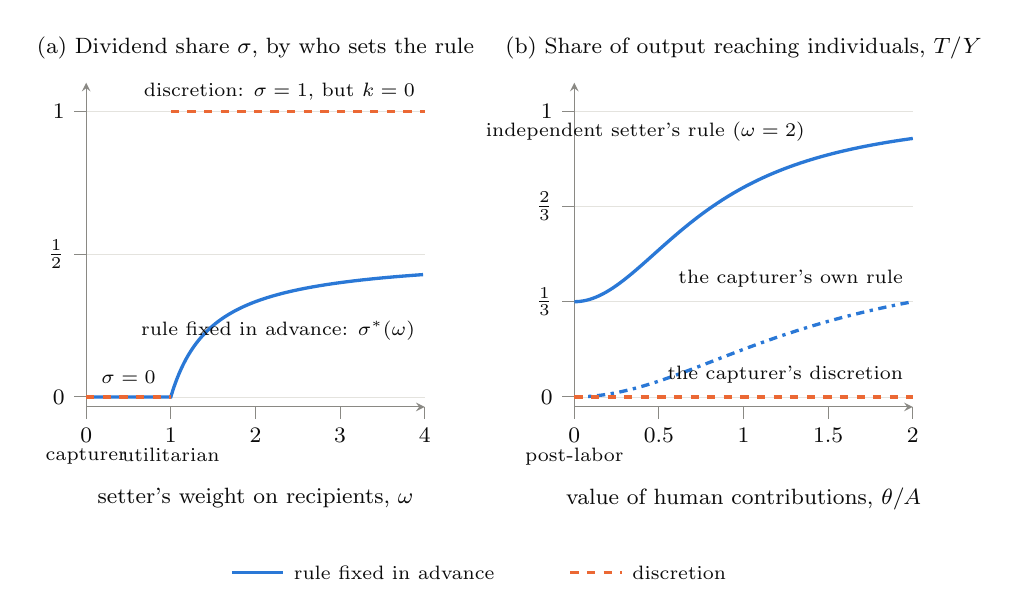
\begin{tikzpicture}
\begin{groupplot}[
    group style={group size=2 by 1, horizontal sep=1.9cm},
    width=0.485\textwidth, height=5.7cm,
    axis lines=left,
    axis line style={line width=0.4pt, draw=axisgray},
    tick style={line width=0.4pt, draw=axisgray},
    tick align=outside,
    ticklabel style={font=\footnotesize, text=ink},
    label style={font=\footnotesize, text=ink},
    title style={font=\footnotesize, text=ink, yshift=-1pt},
    xlabel style={at={(axis description cs:0.5,-0.22)}, anchor=north},
    ymajorgrids, grid style={line width=0.3pt, draw=gridgray},
    clip=false,
]
% ---------------- panel (a)
\nextgroupplot[
    title={(a) Dividend share $\sigma$, by who sets the rule},
    xlabel={setter's weight on recipients, $\omega$},
    xmin=0, xmax=4, ymin=-0.035, ymax=1.1,
    xtick={0,1,2,3,4},
    xticklabels={{\shortstack{0\\[-1pt]{\scriptsize capturer}}},
                 {\shortstack{1\\[-1pt]{\scriptsize utilitarian}}},
                 {\shortstack{2\\[-1pt]{\scriptsize\phantom{y}}}},
                 {\shortstack{3\\[-1pt]{\scriptsize\phantom{y}}}},
                 {\shortstack{4\\[-1pt]{\scriptsize\phantom{y}}}}},
    ytick={0,0.5,1}, yticklabels={$0$,$\tfrac12$,$1$},
]
\addplot[rulec, line width=1.2pt, samples at={0,1,1.02,...,4}]
    {x<=1 ? 0 : (x-1)/(2*x-1)};
\addplot[discc, line width=1.2pt, dashed, domain=0:1, samples=2] {0};
\addplot[discc, line width=1.2pt, dashed, domain=1:4, samples=2] {1};
\node[font=\scriptsize, text=ink, anchor=south east] at (axis cs:4,1.005)
    {discretion: $\sigma=1$, but $k=0$};
\node[font=\scriptsize, text=ink, anchor=north east] at (axis cs:4,0.30)
    {rule fixed in advance: $\sigma^*(\omega)$};
\node[font=\scriptsize, text=ink, anchor=south] at (axis cs:0.5,0.012)
    {$\sigma=0$};
% ---------------- panel (b)
\nextgroupplot[
    title={(b) Share of output reaching individuals, $T/Y$},
    xlabel={value of human contributions, $\theta/A$},
    xmin=0, xmax=2, ymin=-0.035, ymax=1.1,
    xtick={0,0.5,1,1.5,2},
    xticklabels={{\shortstack{0\\[-1pt]{\scriptsize post-labor}}},
                 {\shortstack{0.5\\[-1pt]{\scriptsize\phantom{y}}}},
                 {\shortstack{1\\[-1pt]{\scriptsize\phantom{y}}}},
                 {\shortstack{1.5\\[-1pt]{\scriptsize\phantom{y}}}},
                 {\shortstack{2\\[-1pt]{\scriptsize\phantom{y}}}}},
    ytick={0,0.3333,0.6667,1}, yticklabels={$0$,$\tfrac13$,$\tfrac23$,$1$},
]
\addplot[rulec, line width=1.2pt, domain=0:2, samples=120]
    {(2/9+x^2)/(2/3+x^2)};
\addplot[rulec, line width=1.2pt, dashdotted, domain=0:2, samples=120]
    {(x^2/4)/(1+x^2/2)};
\addplot[discc, line width=1.2pt, dashed, domain=0:2, samples=2] {0};
\node[font=\scriptsize, text=ink, anchor=south east] at (axis cs:1.42,0.86)
    {independent setter's rule ($\omega=2$)};
\node[font=\scriptsize, text=ink, anchor=south east] at (axis cs:2,0.35)
    {the capturer's own rule};
\node[font=\scriptsize, text=ink, anchor=south east] at (axis cs:2,0.012)
    {the capturer's discretion};
\end{groupplot}
% shared legend
\coordinate (L) at ($(group c1r1.south west)!0.5!(group c2r1.south east)+(0,-2.1cm)$);
\draw[rulec, line width=1.2pt] ($(L)+(-3.4,0)$) -- ++(0.65,0)
    node[right, text=ink, font=\scriptsize] {rule fixed in advance};
\draw[discc, line width=1.2pt, dashed] ($(L)+(0.9,0)$) -- ++(0.65,0)
    node[right, text=ink, font=\scriptsize] {discretion};
\end{tikzpicture}
\caption{The two central results. (a) Under discretion the share of autonomous output
assigned to individuals is a corner, and at the upper corner no autonomous output is left
to share (Proposition~\ref{prop:disc}); a rule fixed in advance gives the interior share
$\sigma^*(\omega)$ (Proposition~\ref{prop:rule}). (b) What a capturer shares vanishes as
human contributions lose value (Proposition~\ref{prop:capt}); under a separated rule the
share converges to $\sigma^*$, here $\tfrac13$ (Proposition~\ref{prop:sep}).}
\label{fig:main}
\end{figure}

\subsection{Separation}

\begin{definition}\label{def:sep}
Allocation is \emph{separated} from capture if three conditions hold.
\begin{enumerate}[label=(S\arabic*)]
\item \emph{Precommitment.} The rule is fixed before investments are made, and no one
      can revise or evade it once output is realized.
\item \emph{Observability.} The capturer and individuals observe the rule in force before
      they act.
\item \emph{Independence.} The setter weights recipients above the capturer: $\omega>1$.
\end{enumerate}
\end{definition}

S3 excludes the capturer, and more. A setter that receives part of the capturer's
profit---as owner, creditor or tax authority---acts like a setter with a lower $\omega$.
If its own weights are $(1,\omega_0)$ and it values its stake in profit at $\rho$, it
maximizes $(1+\rho)\Pi+\omega_0U$, which is the problem of a setter with weight
$\omega_0/(1+\rho)$. A large enough stake in what the rule leaves undistributed turns any
setter into a capturer.

\begin{proposition}[Separation]\label{prop:sep}
Let $\omega\neq 1$. The existence dividend $D$ is strictly positive in equilibrium if and
only if S1, S2 and S3 hold. In that case
\begin{equation}
  \sigma^*=\frac{\omega-1}{2\omega-1}<\frac12, \qquad
  D=\frac{\omega(\omega-1)}{(2\omega-1)^2}\,A^2 .
\end{equation}
\end{proposition}

This is the formal content of the claim that capture and allocation must be separated.
No single condition is surprising; the content is in the conjunction. Wanting to
redistribute is not enough: S3 without S1 ends in confiscation. Commitment is not enough:
S1 without S3 is the capturer's own rule. Three remarks keep the result honest.

First, S1 binds recipients as much as owners. Recipients with discretion end at
confiscation. Separation does not hand the division to the other side; it removes the
division from everyone's reach after the fact.

Second, separation is necessary for a dividend, not sufficient for a larger total. Total
surplus under a separated rule exceeds total surplus under the capturer's own rule by
$\theta^2/8-\sigma^{*2}A^2/2$, which is positive when human contributions matter
($\theta/A>2\sigma^*$) and negative when they do not. In the post-labor limit a dividend
costs output, because it discourages investment, and has to be justified by the weight
placed on those who receive it.

Third, the model takes that weight as given. What it establishes is conditional: anyone
who wants individuals to receive part of what machines produce on their own needs all
three conditions, and loses the dividend entirely if one of them fails.

% ----------------------------------------------------------------------------
\section{Extensions}\label{sec:ext}
% ----------------------------------------------------------------------------

\paragraph{Competition.} Let there be $m\ge 2$ capturers, each with the technology above.

\begin{proposition}[Competition]\label{prop:comp}
(i) Under discretion no capturer pays anything, for any $m$. (ii) Under commitment every
capturer sets $\sigma_j=0$. If contributions are non-excludable, so that each one benefits
every capturer, each sets $s_j=1/(m+1)$ and total transfers are
$\bigl(\tfrac{m}{m+1}\bigr)^2\theta^2$. If contributions are excludable, competition
drives $s$ to one and $T=\theta^2$.
\end{proposition}

Competition pays for what can be taken elsewhere. Existence cannot be taken elsewhere, so
no number of capturers produces a dividend. Excludability---an enforceable right to refuse
access to one's data \citep{ArrietaIbarra2018,JonesTonetti2020}---raises what
contributions earn, but it is itself an allocation rule that someone other than the
capturers has to enforce.

\paragraph{Richer rules.} With complete information a setter could replace the
proportional dividend by a fixed claim $F\le A^2/2$ on autonomous output, which leaves
investment undistorted. Shares stand in for what makes fixed claims impractical: the rule
is written before $A$ is known. Nothing in Propositions~\ref{prop:disc}, \ref{prop:capt}
and~\ref{prop:sep} depends on linearity. Under discretion any setter still transfers
nothing or everything; a capturer still pays nothing unconditional, and
bound~\eqref{eq:bound} is proved for arbitrary transfers; a positive claim on autonomous
output still requires S1--S3.

\paragraph{Prices.} The model has one good and no product market. Competition among
capturers may pass autonomous output to buyers through lower prices. That helps those who
still have income to spend. It does not create income for those whose only asset was
their labor.

% ----------------------------------------------------------------------------
\section{Applying the test}\label{sec:test}
% ----------------------------------------------------------------------------

Proposition~\ref{prop:sep} turns into three questions that can be put to any scheme.
\begin{enumerate}[label=Q\arabic*.,leftmargin=2.6em]
\item Once output is realized, can any party that would gain from a different division
      change the rule or evade it?
\item Can those the rule governs verify the rule before they act, and the transfers
      afterwards?
\item Does whoever sets the rule, or can amend it, keep any part of what it leaves
      undistributed?
\end{enumerate}
A scheme passes if the answers are no, yes and no. One that fails is predicted to pay no
dividend on autonomous output in the long run, whatever rate it announces.

\paragraph{Voluntary pledges.} \citet{OKeefe2020} propose that AI developers commit in
advance to donate a share of any very large profits. In the model this is a rule with
$\sigma>0$ written by the capturer. Proposition~\ref{prop:capt}(b) says a profit-maximizing
capturer would not write it, so the pledge has to rest on motives other than profit or on
outside pressure. Either way Q1 and Q3 return the same answer: the party that wrote the
clause keeps the residual, and unless someone else can enforce the clause, the same party
can unwrite it. The authors themselves describe building meaningful monitoring and
enforcement into such a clause as a significant task.

\paragraph{State dividends.} Alaska has paid residents a dividend from the earnings of
its oil-revenue fund since 1982, in an amount set by a formula in statute. In 2016 the
governor vetoed about half of the appropriation, and in 2017 the state Supreme Court held
that the dividend is subject to the ordinary appropriation and veto process
\citep{Wielechowski2017}. The formula is still in statute, but the amount is now decided
in each year's budget. In 2025 the formula implied roughly \$3,900 per person and the
budget paid \$1,000, the smallest dividend in real terms since the program began
\citep{AlaskaPublic2025,AlaskaDOR2025}. The rule is public, so Q2 is
met. But it can be revised every year (Q1), by a legislature that spends whatever is not
distributed (Q3). The state is no exception to the principle: when it keeps the residual,
it is a capturer.

\paragraph{On-chain rules.} A contract with immutable code and public state satisfies S1
and S2 by construction for whatever settles through it, which is why blockchains have been
analyzed as commitment devices \citep{Szabo1997,CongHe2019,HoldenMalani2019}. Ethereum's fee mechanism shows separation
working at scale. Before August 2021, block producers received every transaction fee.
Under EIP-1559 \citep{Buterin2019} a base fee is set by a public formula from the fullness
of earlier blocks and is burned rather than paid to the producer of the block.
\citet{Roughgarden2021} shows why the burn matters: were the base fee paid to the block
producer, producer and user could undo it with a side payment. Capture---the
power to include and order transactions---was separated from the allocation of the fee.
The rule can still change, but only through a fork of the whole network, not at the
discretion of the producers it constrains. The burn accrues to token holders in proportion
to holdings, not to persons; what the example demonstrates is that a capturing party can
be durably excluded from an allocation it used to control.

A protocol that aims to pay persons has more to solve, and the three questions say where.
A contract its deployer can upgrade is a rule the deployer can revise (Q1). An on-chain
rule sees only what settles on-chain, while autonomous output is mostly produced and sold
elsewhere, so a capturer can evade the rule by routing output around it (Q1 again); the
model assumes this measurement problem away. Governance that receives the undistributed
residual is a residual claimant, and Proposition~\ref{prop:capt} applies to it (Q3). And
an existence dividend needs one claim per person: where identities can be fabricated
\citep{Douceur2002,Borge2017}, the dividend goes to whoever fabricates them most cheaply,
which is capture under another name. These are open design problems. The test does not
solve them. It says which of them must be solved before a protocol's stated rate means
anything.

% ----------------------------------------------------------------------------
\section{Limits and conclusion}
% ----------------------------------------------------------------------------

The model is deliberately small. It takes the setter's weight as given, and so does not
say who should hold the power to set the rule or how a setter with $\omega>1$ comes to
exist and stay independent; appointing the setter is itself an allocation decision, the
constitutional problem of \citet{BrennanBuchanan1980} and
\citet{PerssonRolandTabellini1997}. Utility is linear, which understates what is at
stake: with diminishing marginal utility a utilitarian would also choose a dividend, and
the outcome in which individuals receive nothing would cost more than the model
registers. Technology is additive, individuals are identical, and autonomous output is
assumed to be measurable. Irrevocability is an extreme: a rule that can never be revised
can never be corrected, and real designs trade commitment against flexibility
\citep{Rogoff1985}. S1 asks for less than it seems to. A revision that is announced before
the next round of investment, by a setter that still satisfies S3, is simply a new rule
fixed in advance. The results speak to who may revise the rule and when---not the residual
claimant, and not after the fact---rather than to whether revision should be possible at
all.

The wage solved distribution without anyone designing it, because those who needed labor
had to pay those who could withhold it. Whatever replaces the wage will have to be
designed, and the design problem is narrower than it looks. It is not mainly about the
rate. A rate the capturer can revise is zero. A rate the recipients can revise is one,
applied to nothing. A dividend exists only in between, and the in-between exists only
where the rule is fixed in advance, visible to those it governs, and out of the hands of
whoever keeps the remainder. This is a statement about institutions and is silent on
technology: a constitution, an independent agency, or a contract on a public ledger can
each satisfy it, and each can fail it.


% ----------------------------------------------------------------------------
\appendix
\section{Proofs}
% ----------------------------------------------------------------------------

\begin{proof}[Proof of Proposition~\ref{prop:disc}]
With $k$ and $e$ sunk, $\Pi+\omega U=Y-\half k^2-\half\omega\!\int\! e_i^2\,di+(\omega-1)T$,
where $T=\sigma Ak+s\theta E$. Only the last term depends on the rule. If $\omega<1$ the
setter minimizes $T$: $\sigma=0$ whenever $k>0$ and $s=0$ whenever $E>0$. Anticipating
this, the capturer maximizes $Ak-\half k^2$ and chooses $k=A$, and no individual
contributes, since any contribution would be met with $s=0$. If $\omega>1$ the setter
maximizes $T$: $\sigma=1$ whenever $k>0$, so any $k>0$ earns the capturer $-\half k^2<0$
and $k=0$; and $s=1$ whenever $E>0$, so $e=\theta$.
\end{proof}

\begin{proof}[Proof of Proposition~\ref{prop:rule}]
Given $(\sigma,s)$, the capturer maximizes $(1-\sigma)Ak-\half k^2$ and individual $i$
maximizes $s\theta e_i-\half e_i^2$, the dividend being independent of $e_i$. Hence
$k=(1-\sigma)A$ and $e=s\theta$, and substitution gives $\Pi$ and $U$. The setter's
objective is $A^2g(\sigma)+\theta^2h(s)$ with
$g(\sigma)=\half(1-\sigma)^2+\omega\sigma(1-\sigma)$ and
$h(s)=s(1-s)+\half\omega s^2$. Now $g'(\sigma)=(\omega-1)-(2\omega-1)\sigma$ is linear in
$\sigma$. If $\omega\le 1$ then $g'(0)\le 0$ and $g'(1)=-\omega\le 0$, so $g$ is
decreasing and $\sigma^*=0$. If $\omega>1$ then $g$ is strictly concave with $g'(0)>0$,
so $\sigma^*=(\omega-1)/(2\omega-1)\in(0,\half)$. Next, $h'(s)=1-(2-\omega)s$. If
$\omega\le 1$, $h$ is strictly concave and $h'$ vanishes at $s=1/(2-\omega)\le 1$. If
$\omega>1$, $h'(s)\ge\min\{1,\omega-1\}>0$ on $[0,1]$, so $s^*=1$.
\end{proof}

\begin{proof}[Proof of Corollary~\ref{cor:bound}]
The outcome in Proposition~\ref{prop:disc} is the outcome of the fixed rule $(0,0)$ when
$\omega<1$ and of $(1,1)$ when $\omega>1$. Both rules are available under commitment and
neither is optimal, since $s^*(\omega)>0$ and $\sigma^*(\omega)<1$; $g$ and $h$ have
unique maximizers, so the inequality is strict. The two values follow from
Proposition~\ref{prop:rule}.
\end{proof}

\begin{proof}[Proof of Proposition~\ref{prop:capt}]
(a) is Proposition~\ref{prop:disc}(i).

(b) The linear case is Proposition~\ref{prop:rule} with $\omega=0$: $T=s\theta\cdot
s\theta=\theta^2/4$. For general schedules, an individual can secure $t(0)\ge 0$ by
contributing nothing, so $t_i\ge\half e_i^2$ in equilibrium and
$T\ge\half\!\int\! e_i^2\,di\ge\half E^2$. The capturer's profit is therefore at most
$Ak-\half k^2+\theta E-\half E^2\le\half A^2+\half\theta^2$, with equality only if $k=A$,
$e_i=\theta$ and $t_i=\half\theta^2$ for all $i$. The schedule that pays $\half\theta^2$
for a contribution of at least $\theta$ and nothing otherwise attains the bound, ties being
broken in the capturer's favor. A payment
not conditioned on contributions lowers profit one for one, so $D=0$.

(c) Two facts hold at every history. \emph{Security levels:} the capturer secures
$\half A^2$ in every period by choosing $k=A$ and paying nothing, because $\theta E\ge 0$;
an individual secures $0$ by contributing nothing, because transfers are non-negative.
\emph{Joint surplus:} in any period $\Pi_t+U_t=Ak-\half k^2+\theta E-\half\!\int\!
e_i^2\,di\le\half A^2+\theta E-\half E^2\le\half(A^2+\theta^2)$, by Jensen's inequality.
Fix an equilibrium and a history at which the capturer is to pay $T_t$, and let $V$ be its
continuation value from the next period on if it pays. If it pays nothing, its
continuation value is at least $A^2/(2(1-\delta))$. Paying is optimal only if
$-T_t+\delta V\ge\delta A^2/(2(1-\delta))$. Joint surplus and the individuals' security
level give $V\le(A^2+\theta^2)/(2(1-\delta))$. Combining the two inequalities yields
\eqref{eq:bound}.

For the stationary case, let individuals contribute $e=s\theta$ as long as the capturer
has always paid $s\theta e_i$, and nothing after a default. After a default play reverts
to Proposition~\ref{prop:disc}(i), which holds the capturer to its security level, so no
harsher punishment exists \citep{Abreu1988}. On the path the capturer earns
$\half A^2+s(1-s)\theta^2$ per period and owes $s^2\theta^2$ at the payment stage. It pays
if and only if $s^2\theta^2\le\delta s(1-s)\theta^2/(1-\delta)$, that is, $s\le\delta$.
\end{proof}

\begin{proof}[Proof of Proposition~\ref{prop:sep}]
\emph{If.} Proposition~\ref{prop:rule} with $\omega>1$ gives $\sigma^*\in(0,\half)$ and
$k=(1-\sigma^*)A=\omega A/(2\omega-1)$, so $D=\sigma^*Ak>0$ as stated.

\emph{Only if.} Suppose S1 fails. Then the division in force when output is realized is
chosen at that point, and Proposition~\ref{prop:disc} applies: $D=0$ because $\sigma=0$
(if $\omega<1$) or $k=0$ (if $\omega>1$). Suppose S2 fails, so the rule is fixed but
unobserved. Then $k$ cannot respond to the rule actually chosen, and the setter's choice
is a best response to $k$ taken as given \citep{Bagwell1995}. If $k=0$ then $D=0$. If $k>0$,
that best response is $\sigma=0$ when $\omega<1$, and $\sigma=1$ when $\omega>1$, to which
the capturer's best response is $k=0$, a contradiction. So $D=0$ in every equilibrium.
Suppose S3 fails with $\omega<1$. Then $\sigma=0$ under either timing, by
Propositions~\ref{prop:disc} and~\ref{prop:rule}.
\end{proof}

\begin{proof}[Proof of Proposition~\ref{prop:comp}]
Capturer $j$ has output $Ak_j+\theta E_j$ and rule $(\sigma_j,s_j)$. (i) Under discretion
each capturer's payoff falls one for one with its own transfers. (ii) Under commitment
$\sigma_j$ lowers $j$'s profit and affects nothing else, so $\sigma_j=0$. If
contributions are non-excludable, $E_j=E$ for all $j$, an individual maximizes
$\theta e_iS-\half e_i^2$ with $S=\sum_j s_j$, and $e=\theta S$. Capturer $j$ earns
$(1-s_j)\theta^2S$ from contributions, and the first-order condition is $s_j=1-S$ for
every $j$. Hence $s_j=1/(m+1)$, $S=m/(m+1)$ and $T=S\theta\cdot\theta S$. If contributions
are excludable, each individual directs its contribution to the capturer offering the
highest share, and Bertrand competition gives $s=1$, $e=\theta$ and $T=\theta^2$.
\end{proof}

\bibliographystyle{plainnat}
\bibliography{capture-allocation}

\end{document}
